\documentclass{sig-alternate}
%\documentclass[a4paper,10pt]{article}
\usepackage[utf8]{inputenc}
%El template pincha con spanish babel
%\usepackage[spanish]{babel}
\usepackage{amsmath, amssymb, amsfonts}
\usepackage{graphicx}
\usepackage{fancybox}
\usepackage[table]{xcolor}
\usepackage{soul}

\newtheorem{theorem}{Teorema}

\title{Que bien que est\'a esa cola} 

\numberofauthors{4}
\author{
\alignauthor
Pose, Alberto Miguel\\
       \affaddr{Instituto Tecnol\'ogico de Buenos Aires}\\
       \affaddr{Buenos Aires, Argentina}\\
       \email{apose@alu.itba.edu.ar}
\alignauthor
Catalano, Juan Ignacio\\
       \affaddr{Instituto Tecnol\'ogico de Buenos Aires}\\
       \affaddr{Buenos Aires, Argentina}\\
       \email{jcatalan@alu.itba.edu.ar}
\and
\alignauthor 
Palombo, Mart\'in\\
       \affaddr{Instituto Tecnol\'ogico de Buenos Aires}\\
       \affaddr{Buenos Aires, Argentina}\\
       \email{mpalombo@alu.itba.edu.ar}
\alignauthor 
V\'azquez, Santiago Jos\'e\\
       \affaddr{Instituto Tecnol\'ogico de Buenos Aires}\\
       \affaddr{Buenos Aires, Argentina}\\
       \email{savazque@alu.itba.edu.ar}
}

\date{}

\begin{document}

\maketitle

\begin{abstract}
Se estudia el modelo de cola M/M/1 y M/M/2. ABSTRAEME
\end{abstract} 

\newpage

\section{Introducci\'on}

Se analiza el modelo de Cola simple mediante la simulaci\'on por eventos discretos.
La estructura din\'amica de dicha cola se la indica como M/M/$n$/$\infty$/FIFO, o simplemente M/M/$n$.
La M proviene de Markoviano, es decir, los tiempos entre llegadas y entre servicios son variables
aleatorias con distribuci\'on exponencial y los n\'umeros de llegadas y servicios en un cierto
intervalo de tiempo son procesos de Poisson.  Existen $n$ servidores que atiende a los clientes
y pueden haber infinitos de los mismos en la cola. Adem\'as, ocurre que el primer cliente en llegar es el primero en irse.
En este modelo, se asume que los clientes llegan al sistema mediante un proceso de Poisson con una tasa
media de $\lambda$ [clientes/hora] y el servidor atiende a cada cliente con tiempo de servicio exponencialmente
distribuido con media 1/$\mu$. \\
Si el servidor est\'a desocupado y llega un cliente, entonces este se sirve inmediatamente. Si el servidor est\'a
ocupado, entonces el cliente que llega entra en cola. \\
En la secci\'on \ref{sec:mm1} se analiza el modelo de cola M/M/1. Primero, haciendo referencia al
promedio temporal de clientes en la cola en la secci\'on \ref{sec:parte1} y luego
NOSECOMOSELLAMA en la secci\'on \ref{sec:parte2}.
En la secci\'on \ref{sec:mm2} SEBA PONE QUE PASA ACA.
En la secci\'on \ref{sec:conclusiones} se presentan los resultados y las conclusiones obtenidas en el desarrollo del trabajo.
\section{Nos gustan las colas chiquitas}
\label{sec:mm1}

Se comienza analizando el modelo de cola M/M/1.
Se llama $\rho = \dfrac{\mu}{\lambda}$ a la intensidad de tráfico para el sistema M/M/1.
Se asume que $\rho < 1$. Esto resulta razonable, ya que si $\rho \geq 1$, el sistema se vueve inestable y la cantidad
de clientes en el sistema crece indefinidamente.

\subsection{A nadie le gusta perder tiempo haciendo una cola}
\label{sec:parte1}
El promedio temporal de clientes en la cola $L_q$ se define en \eqref{eq:lQ}.

\begin{equation}
\label{eq:lQ}
L_q = \dfrac{1}{T} \int_{0}^{T} q(t) dt
\end{equation}

Se estima $L_q$ en funci\'on de $\rho$. Fijando $\rho$ se realizan simulaciones para estimar $L_q$
con un error menor al $5\%$. Los resultados se muestran en la figura \ref{fig:meanQueue}, cabe destacar
que sucede lo l\'ogico; al aumentar la intensidad de tr\'afico aumenta la cantidad de clientes en cola.\\

\begin{figure}[ht]
\begin{center}
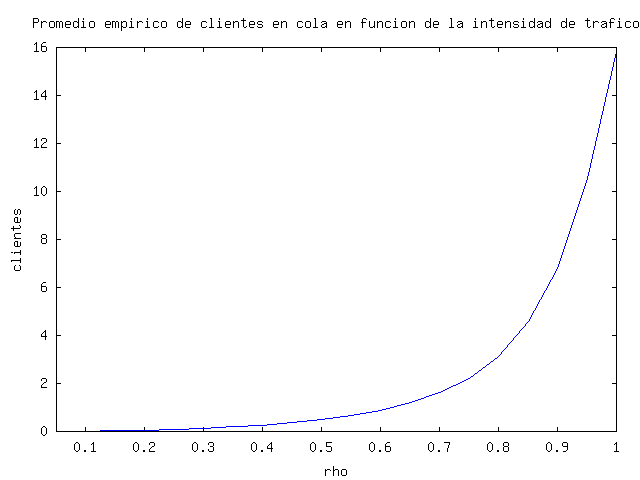
\includegraphics[width=8cm]{queueEmpiricVSrho}
\caption{\label{fig:meanQueue} Promedio temporal emp\'irico de clientes en la cola en funci\'on de $\rho$}
\end{center}
\end{figure}

Se comparan los resultados obtenidos con el valor te\'orico de $L_q$ el cual se ense\~na en \eqref{eq:lQTheoretical}

\begin{equation}
\label{eq:lQTheoretical}
L_q = \dfrac{\rho^{2}}{1 - \rho}
\end{equation}

Los resultados de dicha comparacion se observan en la figura \ref{fig:meanQueueVS}. Se observa que ambas curvas
son casi id\'enticas salvo para los grandes valores de $\rho$ en los cuales se produce una diferencia dr\'astica.
Esto se debe a que para esos casos la simulaci\'on no finaliza al alcanzar un error menor al $5\%$ sino que finaliza
porque alcanza el tope m\'aximo de iteraciones a realizar ($2000$). \'Esto nos dice que para grandes valores de $\rho$
se hace m\'as dif\'icil lograr una buena aproximaci\'on al promedio temporal de clientes en la cola.
CREO QUE SE DEBE A QUE LA VARIANZA TIENE A RHO DANDO VUELTAS PERO NO ME ANIMARIA

\begin{figure}[ht]
\begin{center}
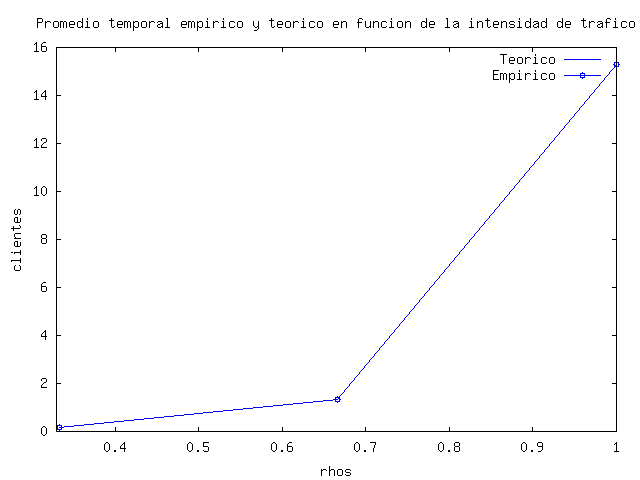
\includegraphics[width=8cm]{teoricoVSempirico}
\caption{\label{fig:meanQueueVS} Comparaci\'on del promedio temporal emp\'irico y te\'orico de clientes en la cola en funci\'on de $\rho$}
\end{center}
\end{figure}

\newpage

\subsection{PARTE2}
\label{sec:parte2}

\section{PARTE3}
\label{sec:mm2}

\section{Resultados y Conclusiones}
\label{sec:conclusiones}
CONCLUIME

% TODO ver si corresponde
% \begin{thebibliography}{10}
% \bibitem{chiTable} Tabla $\chi^{2}$.
% \begin{verbatim}
% http://www.wiphala.net/research/manual/
% statistic/chi_cuadrado.html
% \end{verbatim}
% \bibitem{KSTable} Tabla Kolmogorov-Smirnov.
% \begin{verbatim}
% http://www.eridlc.com/onlinetextbook/
% appendix/table7.htm
% \end{verbatim} 
% \bibitem{TStudentTable} Tabla T Student. \begin{verbatim}www.elosiodelosantos.com/sergiman/archivos/tablat.xls\end{verbatim}
% \end{thebibliography}
\end{document}